All code anchors below refer to the canonical repository
(\texttt{src/ask/…}) and were verified in the pipeline reconstruction
audit (\texttt{docs/audit/CONTROLLERRUN\_RECONSTRUCTION.md}).

\section{4.1 Architectural overview}\label{architectural-overview}

The controller surrounds a SQLite-backed memory store with a governed
write path: per-turn extraction of typed candidates, relation
classification against retrieved priors, a scored three-action policy,
transition execution with lineage, and retrieval/answer stages that
consume only governed state. The per-session flow is driven by
\texttt{ControllerOrchestrator.answer()}
(\texttt{src/ask/pipeline/orchestrator.py}).

\begin{figure}
\centering
\pandocbounded{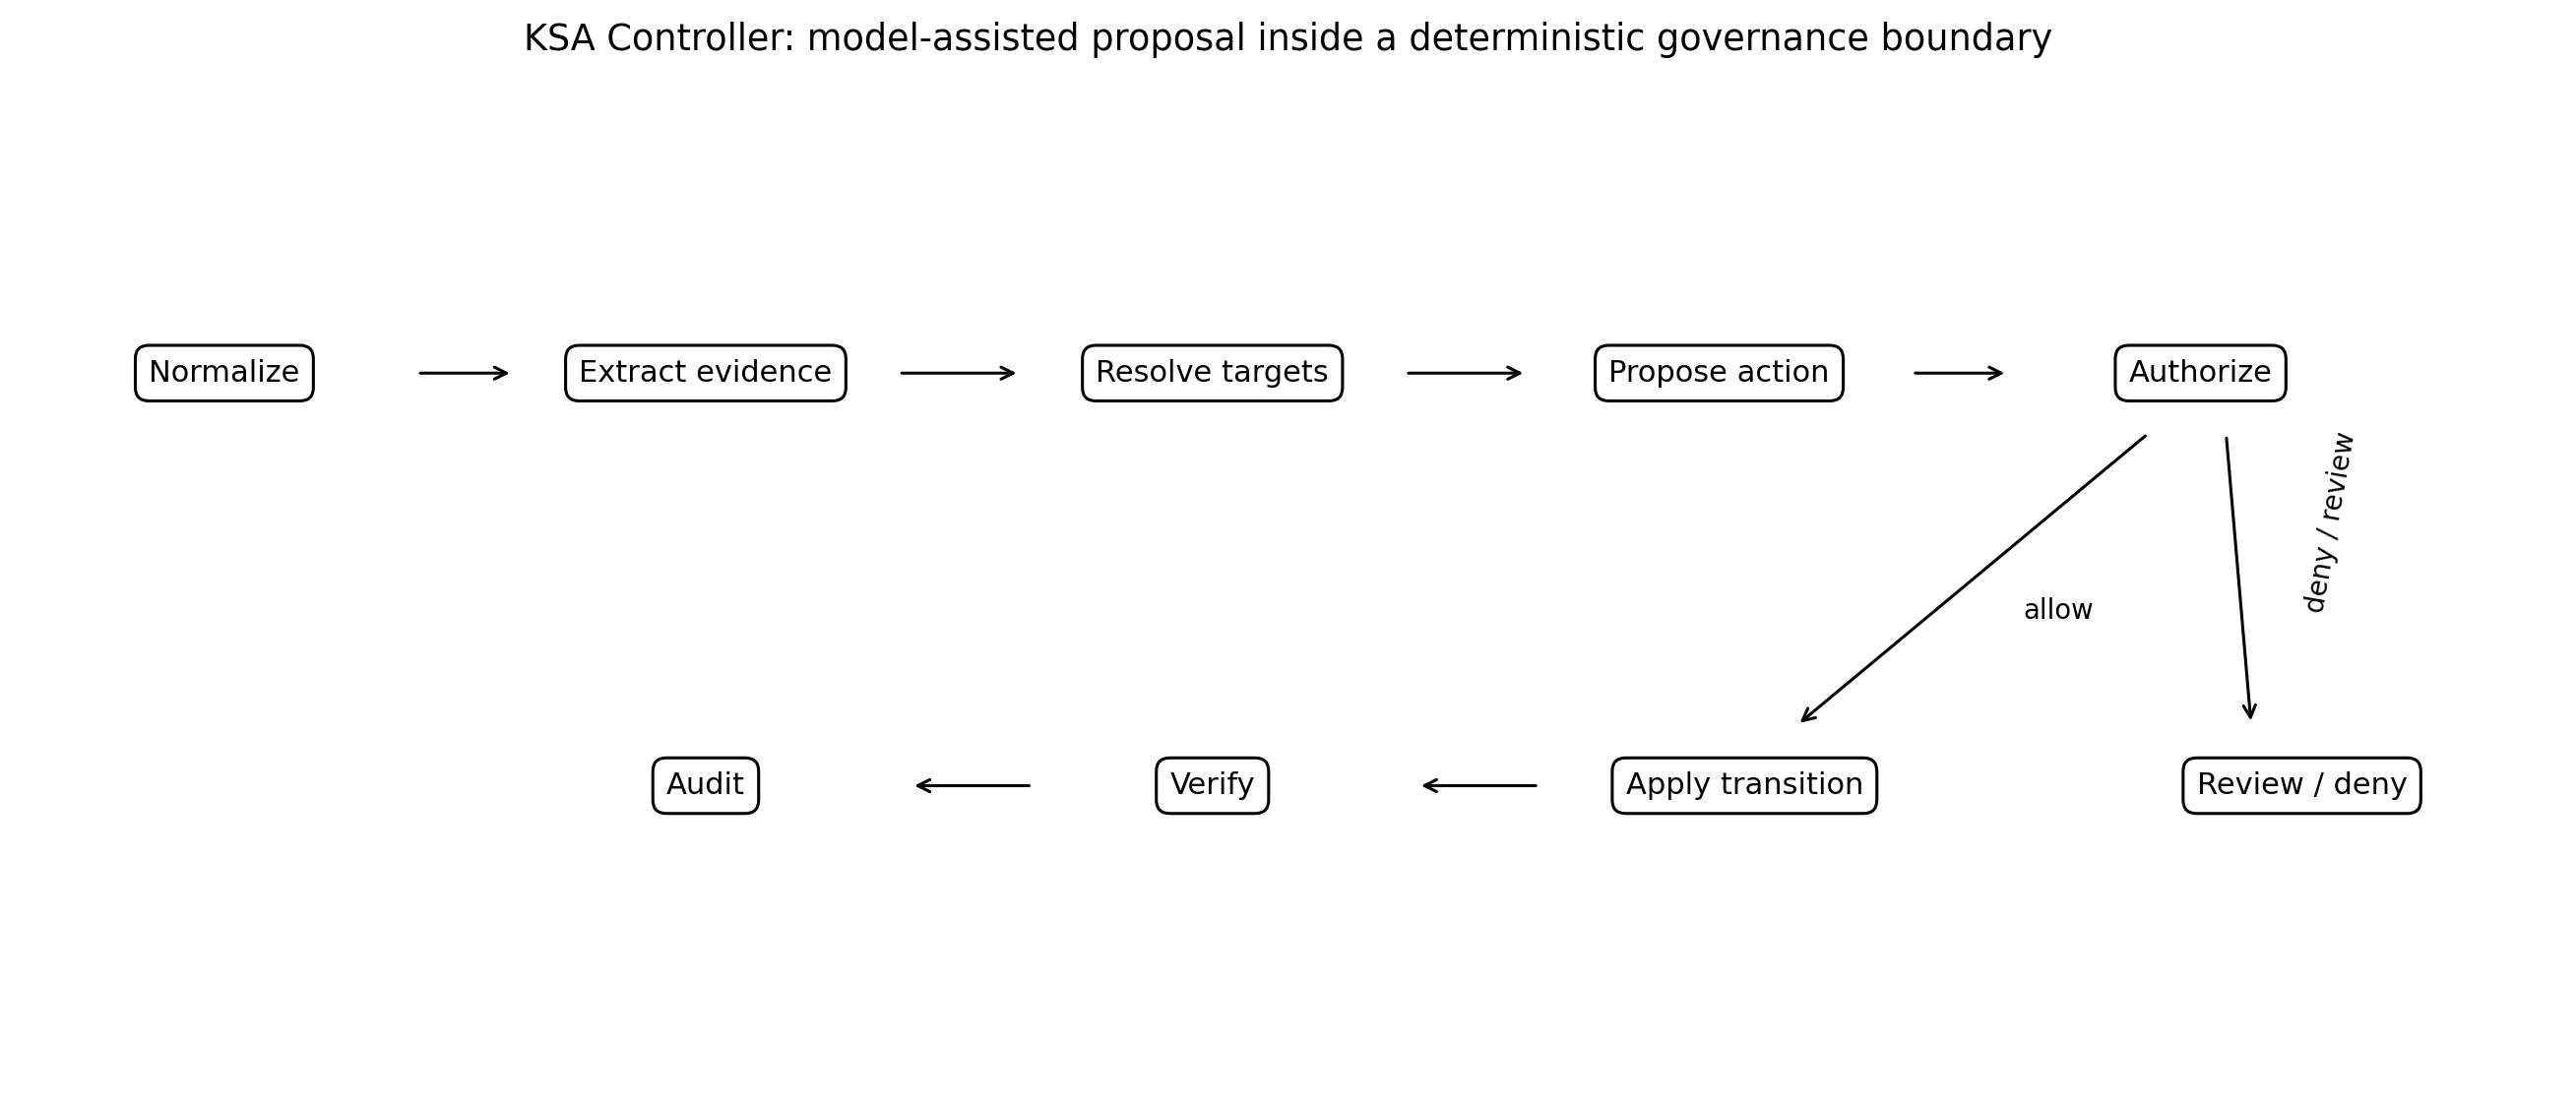
\includegraphics[keepaspectratio]{../../docs/figures/figure_07_ask_controller_architecture.png}}
\caption{ASK Controller architecture.}
\end{figure}

\begin{Shaded}
\begin{Highlighting}[]
\NormalTok{User turns}
\NormalTok{   |}
\NormalTok{   v}
\NormalTok{[Extractor (strict JSON schema)] {-}{-}\textgreater{} typed candidate memories}
\NormalTok{   |}
\NormalTok{   v}
\NormalTok{[Prefilter: top{-}64 turns by question similarity]}
\NormalTok{   |}
\NormalTok{   v}
\NormalTok{[Relation classifier (two{-}stage, optional escalation)]}
\NormalTok{   |            candidate vs selected prior}
\NormalTok{   v}
\NormalTok{[Policy: scored KEEP / SUPERSEDE / ABSTAIN]}
\NormalTok{   |}
\NormalTok{   v}
\NormalTok{[Memory operations: insert\_active | supersede(+lineage) | no{-}op]}
\NormalTok{   |}
\NormalTok{   v}
\NormalTok{[Retrieval over active records (dense, k=16, neighbor expansion)]}
\NormalTok{   |}
\NormalTok{   v}
\NormalTok{[Answer{-}context compilation (session{-}diverse rerank, \textasciitilde{}12k{-}token budget)]}
\NormalTok{   |}
\NormalTok{   v}
\NormalTok{[Answerer]  {-}{-}\textgreater{}  [Judge / grader with guarded normalization]}
\end{Highlighting}
\end{Shaded}

\section{4.2 Extraction}\label{extraction}

\texttt{Extractor.render\_prompt()} renders a per-turn extraction prompt
bound to a strict JSON schema
(\texttt{ExtractionOutput.model\_json\_schema()});
\texttt{Extractor.extract()} is called per user turn, concurrently
(default concurrency 8). Extraction is fail-closed as of v8: on a
provider no-response the extractor raises rather than caching a
fabricated empty extraction --- the v7 behavior of caching empties is
the documented contamination source F1/F2 (§7.6). A content-keyed shared
extraction cache allows cross-run reuse without re-introducing synthetic
empties.

\section{4.3 Relation classification and prior
selection}\label{relation-classification-and-prior-selection}

For each candidate, \texttt{\_process\_candidate()} runs a two-stage
relation classifier (\texttt{RelationClassifier.classify()}) with an
optional cascade escalation to a stronger model --- gated so that
escalation is a no-op unless a genuinely different model is configured
(the v7 run set \texttt{BIG\_MODEL\ ==\ FAST\_MODEL}, making its
escalation tier inert; disclosed in §7.6). Prior selection
(\texttt{\_find\_prior}, \texttt{\_select\_prior\_relation}) picks the
stored record against which the relation is evaluated.

\section{4.4 Prototype scorecard and released reference
policy}\label{prototype-scorecard-and-released-reference-policy}

\texttt{controller.policy.decide()} implements the scored three-action
rule:

\begin{Shaded}
\begin{Highlighting}[]
\NormalTok{if S\_abstain  \textgreater{} \ensuremath{\theta}\_abs:                          ABSTAIN}
\NormalTok{elif S\_revise \textgreater{} \ensuremath{\theta}\_sup and relation\_update \textgreater{} 0:  SUPERSEDE}
\NormalTok{else:                                           KEEP}
\end{Highlighting}
\end{Shaded}

with feature scoring in \texttt{src/ask/controller/scoring.py}. The
features are deliberately few and human-legible (a five-feature
scorecard over relation evidence, type compatibility, provenance
agreement, and conflict signals), so a runtime decision can be explained
by inspection of its feature values.

This runtime scorecard did \textbf{not} generate the released MGP-6
reference predictions. Those predictions came from the deterministic
lexical predicate policy in
\texttt{benchmarks/mgp6/systems/policies.py}. Chapter 7 therefore
evaluates that artifact as a \emph{reference policy}, not as evidence
for the five-feature scorecard or its thresholds. The scorecard remains
an implemented architectural option whose independent tuning and
evaluation are open work.

\section{4.5 The LLM policy and the decision
baselines}\label{the-llm-policy-and-the-decision-baselines}

The LLM-backed controller replaces the scorecard with a model decision
(qwen/qwen3.5-9b) inside the same scaffold: same extraction, relation
evidence, action vocabulary, and transition semantics. Two decision
baselines isolate the contribution of the scaffold itself: a zero-shot
LLM decision baseline (no governance framing; 0.700 accuracy,
invalid-commit 0.606) and a six-shot run with 174/180 predictions. The
latter is scored coverage-aware by aligning the six missing IDs as
INVALID (accuracy 0.7833; macro-F1 0.7692) and remains
\texttt{incomplete}, not a completed-run comparison (§7.2).

\section{4.6 Memory operations and
lineage}\label{memory-operations-and-lineage}

\texttt{src/ask/memory/operations.py} implements
\texttt{insert\_active}, \texttt{supersede} (links lineage, marks the
prior inactive), \texttt{supersede\_evict}, \texttt{retrieve\_active}
(excludes superseded records), and \texttt{get\_lineage}. Lineage is
what makes supersession auditable: the losing record remains queryable
with its link to the superseding record, rather than being deleted or
silently overwritten --- the same auditability argument made formally by
TOKI's audit rows \citep{wang2026toki} and operationally by Zep's
invalidation timestamps \citep{rasmussen2025zep}, here scored directly
via the lineage-integrity metric.

\section{4.7 Retrieval and answer-context
compilation}\label{retrieval-and-answer-context-compilation}

Retrieval is dense (MiniLM-L6-v2, max sequence length 256, k=16) with
neighbor expansion (±2 turns), assistant/raw-user context pools, and
query-gated historical lineage (historical context is offered only when
the question requests history). Answer-context compilation reranks for
the answer, applies cross-session diversity (v8), and trims to a
\textasciitilde12,000-token budget. The answerer (qwen3.5-9b,
temperature 0) uses per-competency prompts with a WORK→FINAL scaffold.
These retrieval-side mechanisms matter for Chapter 8: grounding supply
is the dominant failure family in the contaminated v7 SSP diagnostic,
while the later top-up shows that results cannot be carried across
configurations.

\section{4.8 Judging and normalization}\label{judging-and-normalization}

\texttt{LongMemEvalGrader.grade()} applies ordered guards (blank,
degenerate, refusal, abstention) before the token guard;
\texttt{\_normalize\_text()} collapses spelled-out cardinals and
multiplicatives (``twice''→``2''); the hard gold-token reject fires only
on a provable numeric conflict, with all lexical/entity/date mismatches
deferred to the semantic LLM judge. These fixes respond to documented
judge false negatives (F6, §8.3) and are themselves part of the audit
trail.

\section{4.9 Test strategy}\label{test-strategy}

Unit and regression tests cover fail-closed extraction
(\texttt{test\_extractor\_recovery.py}), decision semantics, lineage
operations, merge-by-session-id de-duplication
(\texttt{merge\_run\_shards()}), and the guard logic above. The primary
standalone, stdlib-only analysis
(\texttt{scripts/analysis/audit\_mgp6\_validity.py}) recomputes shortcut
probes, held-out metrics, cluster intervals, finite-sample bounds,
calibration, risk--coverage, and cost sensitivity from per-item
predictions. The older \texttt{mcnemar\_mgp6.py} item-level analysis
remains reproducible but secondary (Appendix E).

\section{4.10 Operational modes}\label{operational-modes}

The controller supports simulation (no mutation), shadow, assisted
(human approval for selected actions), and autonomous modes; ABSTAIN
routes to review rather than committing. Deployment guidance (Chapter 9)
restricts autonomous supersession to policy-stable, well-audited cases.
